\documentclass[11pt]{article}
\usepackage[a4paper,margin=2.2cm]{geometry}
\usepackage{graphicx}
\usepackage{caption}
\usepackage[colorlinks=true,linkcolor=blue,urlcolor=blue]{hyperref}
\captionsetup{font=small,labelfont=bf}
\title{Supplementary material for\\
Mother-pebble-resolved fracture sequences in random Li$_4$SiO$_4$ ceramic breeder beds by bonded-template DEM}
\author{Jian Wang et al.}
\date{}

\begin{document}
\maketitle

\begin{figure}[ht]
\centering
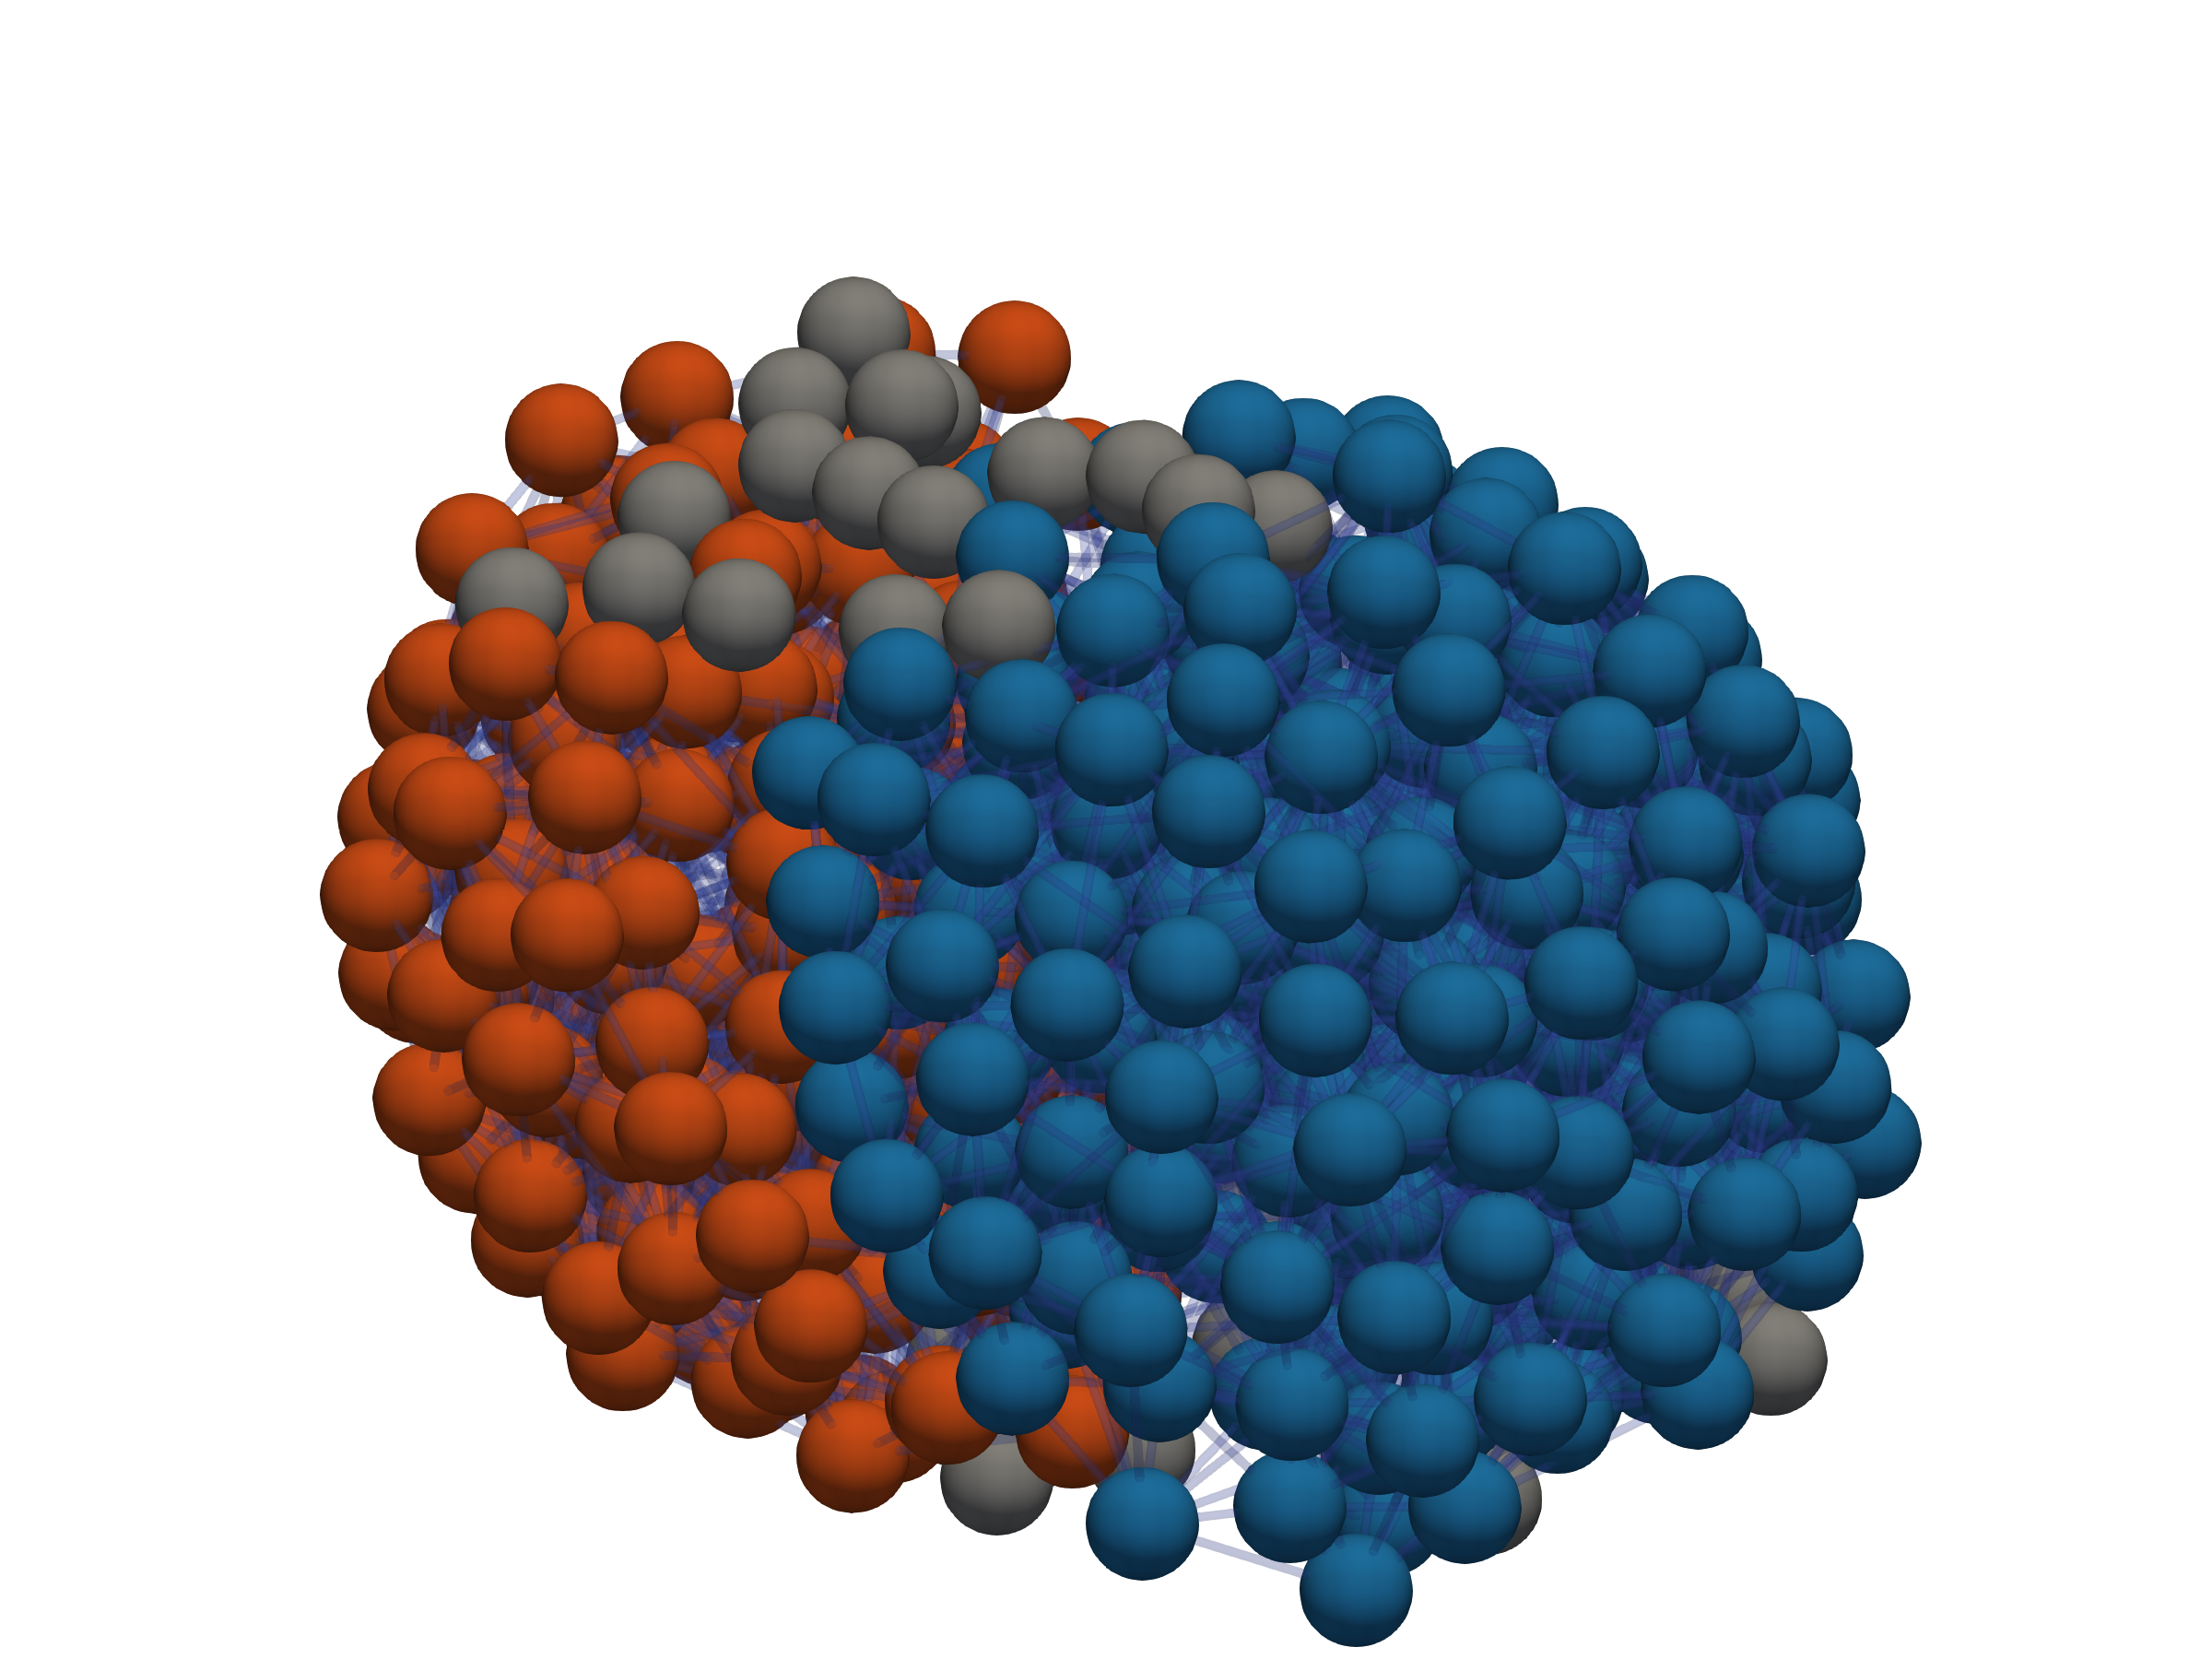
\includegraphics[width=0.86\textwidth]{../figures/sp002/single_pebble_fragment_morphology_paraview.png}
\caption*{\textbf{Supplementary Fig. S1 | Three-dimensional single-pebble fragment morphology.}
Final morphology of the x-normal 0.05 m s$^{-1}$ single-pebble rerun at 0.30 mm displacement, rendered from the particle and intact-bond dumps. The 500 subparticles are coloured by final intact-bond connected component: largest fragment, second-largest fragment and smaller fragments. Semi-transparent tubes show the remaining intact internal bonds. The final graph contains 5335 intact bonds and 40 fragments, with the two largest fragments containing 236 and 226 subparticles. The split-type morphology is used as qualitative calibration evidence against published Li$_4$SiO$_4$ single-pebble fracture observations.}
\end{figure}

\end{document}
